\section{Support Vector Shape (SVS)}
\label{sec:bg_svs}
Support Vector Shape (SVS) introduces an implicit 2D or 3D shape discrimination based on Support Vector Machine (SVM) \cite{Nguyen2013}. Shapes are defined as decision function from training SVM with Radial Basis Function (RBF) kernel. SVS representation introduces several powerful advantages:
\begin{itemize}
  \item Expressing shapes against noise, fragmentation and artifacts.
  \item Presenting shapes with invariance of scale, rotation and translation.
  \item Producing shapes features reliably.
\end{itemize}

\subsection{Training Decision Function}
SVS shape descriptor involves SVM to learn decision function that will be able to distinguish points from whether they lies in given shape with a probability. To represent shapes with continuous function, SVM with RBF kernel gives an analytical solution. RBF kernel function can map data with arbitrary features to an infinite-dimension space where given shape can be linear separated from other points. The decision function of SVS is defined as \cite{Nguyen2013}:
\begin{equation}
\label{eq:svsdf}
f(x)=\sum^m_{i=1}\alpha_i[\Phi(x).\Phi(x^*_i)]
\end{equation}
where $x^*_i$ are support vectors with corresponding weight $\alpha_i$ and $\Phi$ is a mapping function in product space $H$ where the RBF kernel function replaces the dot product as:
\begin{equation}
\label{eq:svskernel}
k(x,x^*_i)=\Phi(x).\Phi(x^*_i)=exp(-\gamma||x-x^*_i||^2)
\end{equation}
Combining equation \ref{eq:svsdf} and \ref{eq:svskernel} gives a comprehensive expression:
\begin{equation}
\label{eq:svs}
f(x)=\sum^m_{i=1}\alpha_iexp(-\gamma||x-x^*_i||^2)
\end{equation}

For training SVS, arbitrary points lies in shapes are chosen as positive training samples, while random external points that close to shape contour are sampled as negative training set. Lastly, v-SVM \cite{scholkopf2001estimating} are employed to learn the decision function to separate positive and negative points.

\begin{figure}[h]
    \centering
    \begin{subfigure}[b]{0.5\textwidth}
        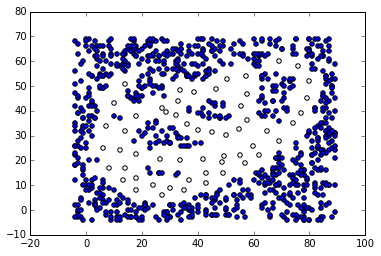
\includegraphics[width=\textwidth]{resources/Background/svs_samples} 
        \caption{Sampled Positive(white) and Negative(blue) Points}
        \label{fig:svs1}
    \end{subfigure}
    \hfill
    \begin{subfigure}[b]{0.4\textwidth}
        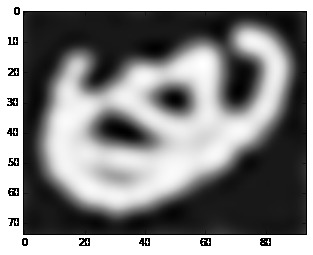
\includegraphics[width=\textwidth]{resources/Background/trained_svs} 
        \caption{Trained SVS Shape}
        \label{fig:svs2}
    \end{subfigure}
    \caption{SVS Training Points and Trained Shape}
\end{figure}

Figure \ref{fig:svs1} shows the training points where blue and white are marked as negative and positive respectively. Figure \ref{fig:svs2} revealed the final trained SVS plot, in which write colour means points are considered as part of shape with high possibility while black colour means the opposite.

\subsection{SVS Feature Points}
With SVS shape representation, reliable scale, rotation and translation invariant feature points can be retrieved based on decision function \ref{eq:svs}. Four types of feature points are produced by SVS representation: gradient based, support vector based, curvature based and entropy based feature points.

\subsubsection{Gradient Based Feature}
The gradient feature is reliable because gradient orientation is stable while gradient magnitude differs by constant factors. Gradient can be found by finding first derivative of $f(x)$ \cite{Nguyen2013}:
\begin{equation}
\label{eq:svsgrad}
\nabla f(x)=2\gamma\sum^m_{i=1}\alpha_iexp(-\gamma||x-x^*_i||^2)(x^*_i-x)
\end{equation}
where gradient orientation given by $\frac{\nabla f(X)}{||\nabla f(X)||}$. Experiments in \cite{Nguyen2013} shows gradient is stable for higher gradient magnitude points.

\subsubsection{Support Vector Based Feature}
Support vectors are claimed suitable to be feature points on it selves, due to their discriminative power of training decision function and gradient. But support vectors are sensitive to object shape. Shape deformation affects support vectors significantly.

\subsubsection{Curvature Based Feature}
Curvature based features tend to calculate points with sharp curves on decision function. Especially for 2D situation, eigenvalues of Hessian matrix is close related to curvature value:
\begin{equation}
\label{eq:svshessian}
H=
\begin{bmatrix}
    \frac{\partial^2f}{\partial x^2_1} & \frac{\partial^2f}{\partial x_1\partial x_2}\\
    \frac{\partial^2f}{\partial x_1\partial x_2} & \frac{\partial^2f}{\partial x^2_2}
\end{bmatrix}
=Q
\begin{bmatrix}
    \lambda_1 & 0\\
    0 & \lambda_2
\end{bmatrix}
Q^{-1}
\end{equation}
where points $(x_1,x_2)$ having large curvature associated with large eigenvalue in both dimension. Curvature features are highly discriminative but is not appropriate for shape matching.

\subsubsection{Entropy Based Feature}
Another similar measurement for selecting feature points is using entropy of local gradient orientation. The entropy is computed as \cite{Nguyen2013}:
\begin{equation}
\label{eq:svsentropy}
-\sum_{i=1}^np_i\log_2(p_i)
\end{equation}
where $p_i$ is the weight of bin $i$ and $n$ is number of bins in histogram. High entropy is proportional to gradient directional variation. The feature also provides highly reliable descriptor but are difficult to compute in higher dimension.